\documentclass{article} % For LaTeX2e
\usepackage{nips13submit_e,times}
\usepackage{hyperref}
\usepackage{url}
\usepackage{graphicx}
%\documentstyle[nips13submit_09,times,art10]{article} % For LaTeX 2.09


\title{  Extracting and Aggregating Aspect-Level Sentiment from Product Reviews  }


\author{
Matthew Long, Desmond C. Ong, Shane Soh \\
Stanford University \\
\texttt{\{mlong14, dco, shanesoh\}@stanford.edu}
%Matthew Long \\
%Stanford University\\
%\texttt{mlong14} \\
%\And
%Desmond C. Ong \\
%%Psychology \\
%Stanford University \\
%\texttt{dco} \\
%\And
%Shane Soh \\
%%Affiliation \\
%Stanford University \\
%\texttt{shanesoh} \\
}

% The \author macro works with any number of authors. There are two commands
% used to separate the names and addresses of multiple authors: \And and \AND.
%
% Using \And between authors leaves it to \LaTeX{} to determine where to break
% the lines. Using \AND forces a linebreak at that point. So, if \LaTeX{}
% puts 3 of 4 authors names on the first line, and the last on the second
% line, try using \AND instead of \And before the third author name.

\newcommand{\fix}{\marginpar{FIX}}
\newcommand{\new}{\marginpar{NEW}}

\nipsfinalcopy % Uncomment for camera-ready version

\begin{document}


\maketitle

\begin{abstract}
Previous work in \textit{aspect-level sentiment analysis}---identifying the sentiment associated with products and their individual attributes, like battery life---have mostly been formulated as supervised learning problems, requiring known labels of both the relevant aspects and their sentiment. Here we propose a hybrid method where we first generate aspects from natural language text via unsupervised clustering of word vector representations, and secondly extract aspect-level sentiment. We further propose a deep learning architecture for aggregating and summarizing these aspect-level sentiment within and across reviews.
\end{abstract}

\section{Introduction}

In today's e-commercialized society, the consumer not only has access to online stores through which she might purchase anything she desires, but she also has unprecedented access to a deluge of information---most notably, product reviews written by other consumers---with which she can make her decision. Unfortunately, sifting through hundreds of reviews across tens of different websites to acquire specific information about the product and its important attributes (e.g. \textit{battery life} for electronics) is a time-consuming chore. Because of this, there has been much recent research tackling the two separate but connected components of this problem: (1) entity-level or aspect-specific sentiment analysis, and (2) summarization and aggregation of reviews.

Within the context of a product review, the first component, \textit{aspect-specific sentiment analysis}, involves identifying individual ``aspects" (which could be the product itself, or features/attributes of the product), and subsequently identifying the sentiment---positive, neutral, or negative judgments---associated with those aspects [1-5]. Previous methods have relied on graphical models (e.g. Latent Dirichlet Allocation [1-3], Conditional Random Fields [4]), or directly modeling sentiment compositionality [5]. In this paper, we propose extending recent successful advances in deep learning [6-7] to address this problem. In particular, we seek to improve and extend the work in [7], who propose using several deep learning architectures like the Recursive Neural Tensor Network (RNTN) to extract aspect and sentiment in a single step. Most of the previous work mentioned [1-2,4-7] (except [3]) are supervised methods that require labeled aspects-sentiment pairs for training. This is unscalable, and a better approach would be to automatically identify relevant aspects for each product. This is made more difficult by the fact that relevant aspects might differ across similar products. For example, for a given electronic item such as a mobile phone, relevant aspects could be the battery life, screen size, weight, cost, and more. Not all these aspects are relevant across other electronic items: for a computer, weight might not be an issue, and screen size might be moot for headphones. We propose using unsupervised methods to generate candidate aspects via semantic word vector representations, followed by simultaneous extraction of aspect and sentiment.

The second problem involves aggregation of reviews, or constructing a \textit{meta-review}. Previous work [8-10] has shown that simple averaging of the ``stars" of reviews for an individual product is sub-optimal. Here we propose a deep learning architecture to aggregate the previously identified aspect-specific sentiment across multiple sentences within a review, and furthermore, to aggregate these sentiment across multiple reviews.










\section{Problem Statement}
%Describe your problem precisely specifying the dataset to be used, expected results and evaluation

Our proposed workflow can be divided into three main parts: {\bf Aspect Identification}, {\bf Aspect-Specific Sentiment Extraction}, and {\bf Sentiment Aggregation}. See Fig. \ref{workflow} for an illustration.

\subsection{Aspect Identification}

\textbf{Problem}: Given an {\bf unlabeled} set of product reviews (for a single product), identify clusters $\{C_1,\ldots, C_k\}$, where the (weighted) centroid of cluster $i$ would represent aspect $i$, and member words of cluster $i$ would represent synonyms that map onto the same aspect $i$.

\textbf{Dataset}: Amazon Reviews of Electronics [11] {\it \bf (fill in how many reviews)}.

\textbf{Evaluation}: {\it \bf (fill in)}.

\subsection{Aspect-Specific Sentiment Extraction}

\textbf{Input}: From above, we can generate aspect labels for product reviews. We will also use an existing trained sentiment analysis model to generate sentiment labels for each token / unigram.

\textbf{Problem}: Given a set of product reviews (for a single product), identify (aspect, aspect-related sentiment) tuples. This is a similar problem statement as [7]: we intend to expand upon their model.

\textbf{Evaluation}: {\it \bf (fill in)}.

\subsection{Aspect-Specific Sentiment Aggregation}

\textbf{Input}: From above, we have (aspect, aspect-related sentiment) tuples which come from multiple sentences within a review, and across multiple reviews, for a given product.

\textbf{Dataset}: We propose scraping some product reviews off Consumer Reports (or similar sites like CNET.com, or DPReview for Cameras) to collect a small, labeled dataset. These websites provide professionally produced aspect-related sentiment ratings, which we take to be the gold standard.

\textbf{Problem}: Given a set of (aspect, aspect-related sentiment) tuples (for a single product), optimally summarize them into a ``meta-review". The desired output is a sentiment-aspect vector where the $i$-th element is the sentiment for aspect $i$. We plan to scrape a small set of labeled summaries, and use a semi-supervised recursive neural network architecture (or a variant) to learn how to compositionally combine individual (aspect, aspect-related sentiment) tuples.% to generate a single vector of summarized aspect-related sentiment.

\textbf{Evaluation}: We will set aside some of the labeled gold standard meta-reviews into dev and test sets. We will report accuracy on the dev sets (e.g. L2 distance between the predicted and actual sentiment vectors) as a function of training set-size (increased in a semi-supervised manner) and other hyper parameters. Finally, we will report accuracy on the test set.


\section{Technical Approach and Models} 
%Describe the methods you intend to apply to solve the given problem

\begin{figure}[h]
\begin{center}
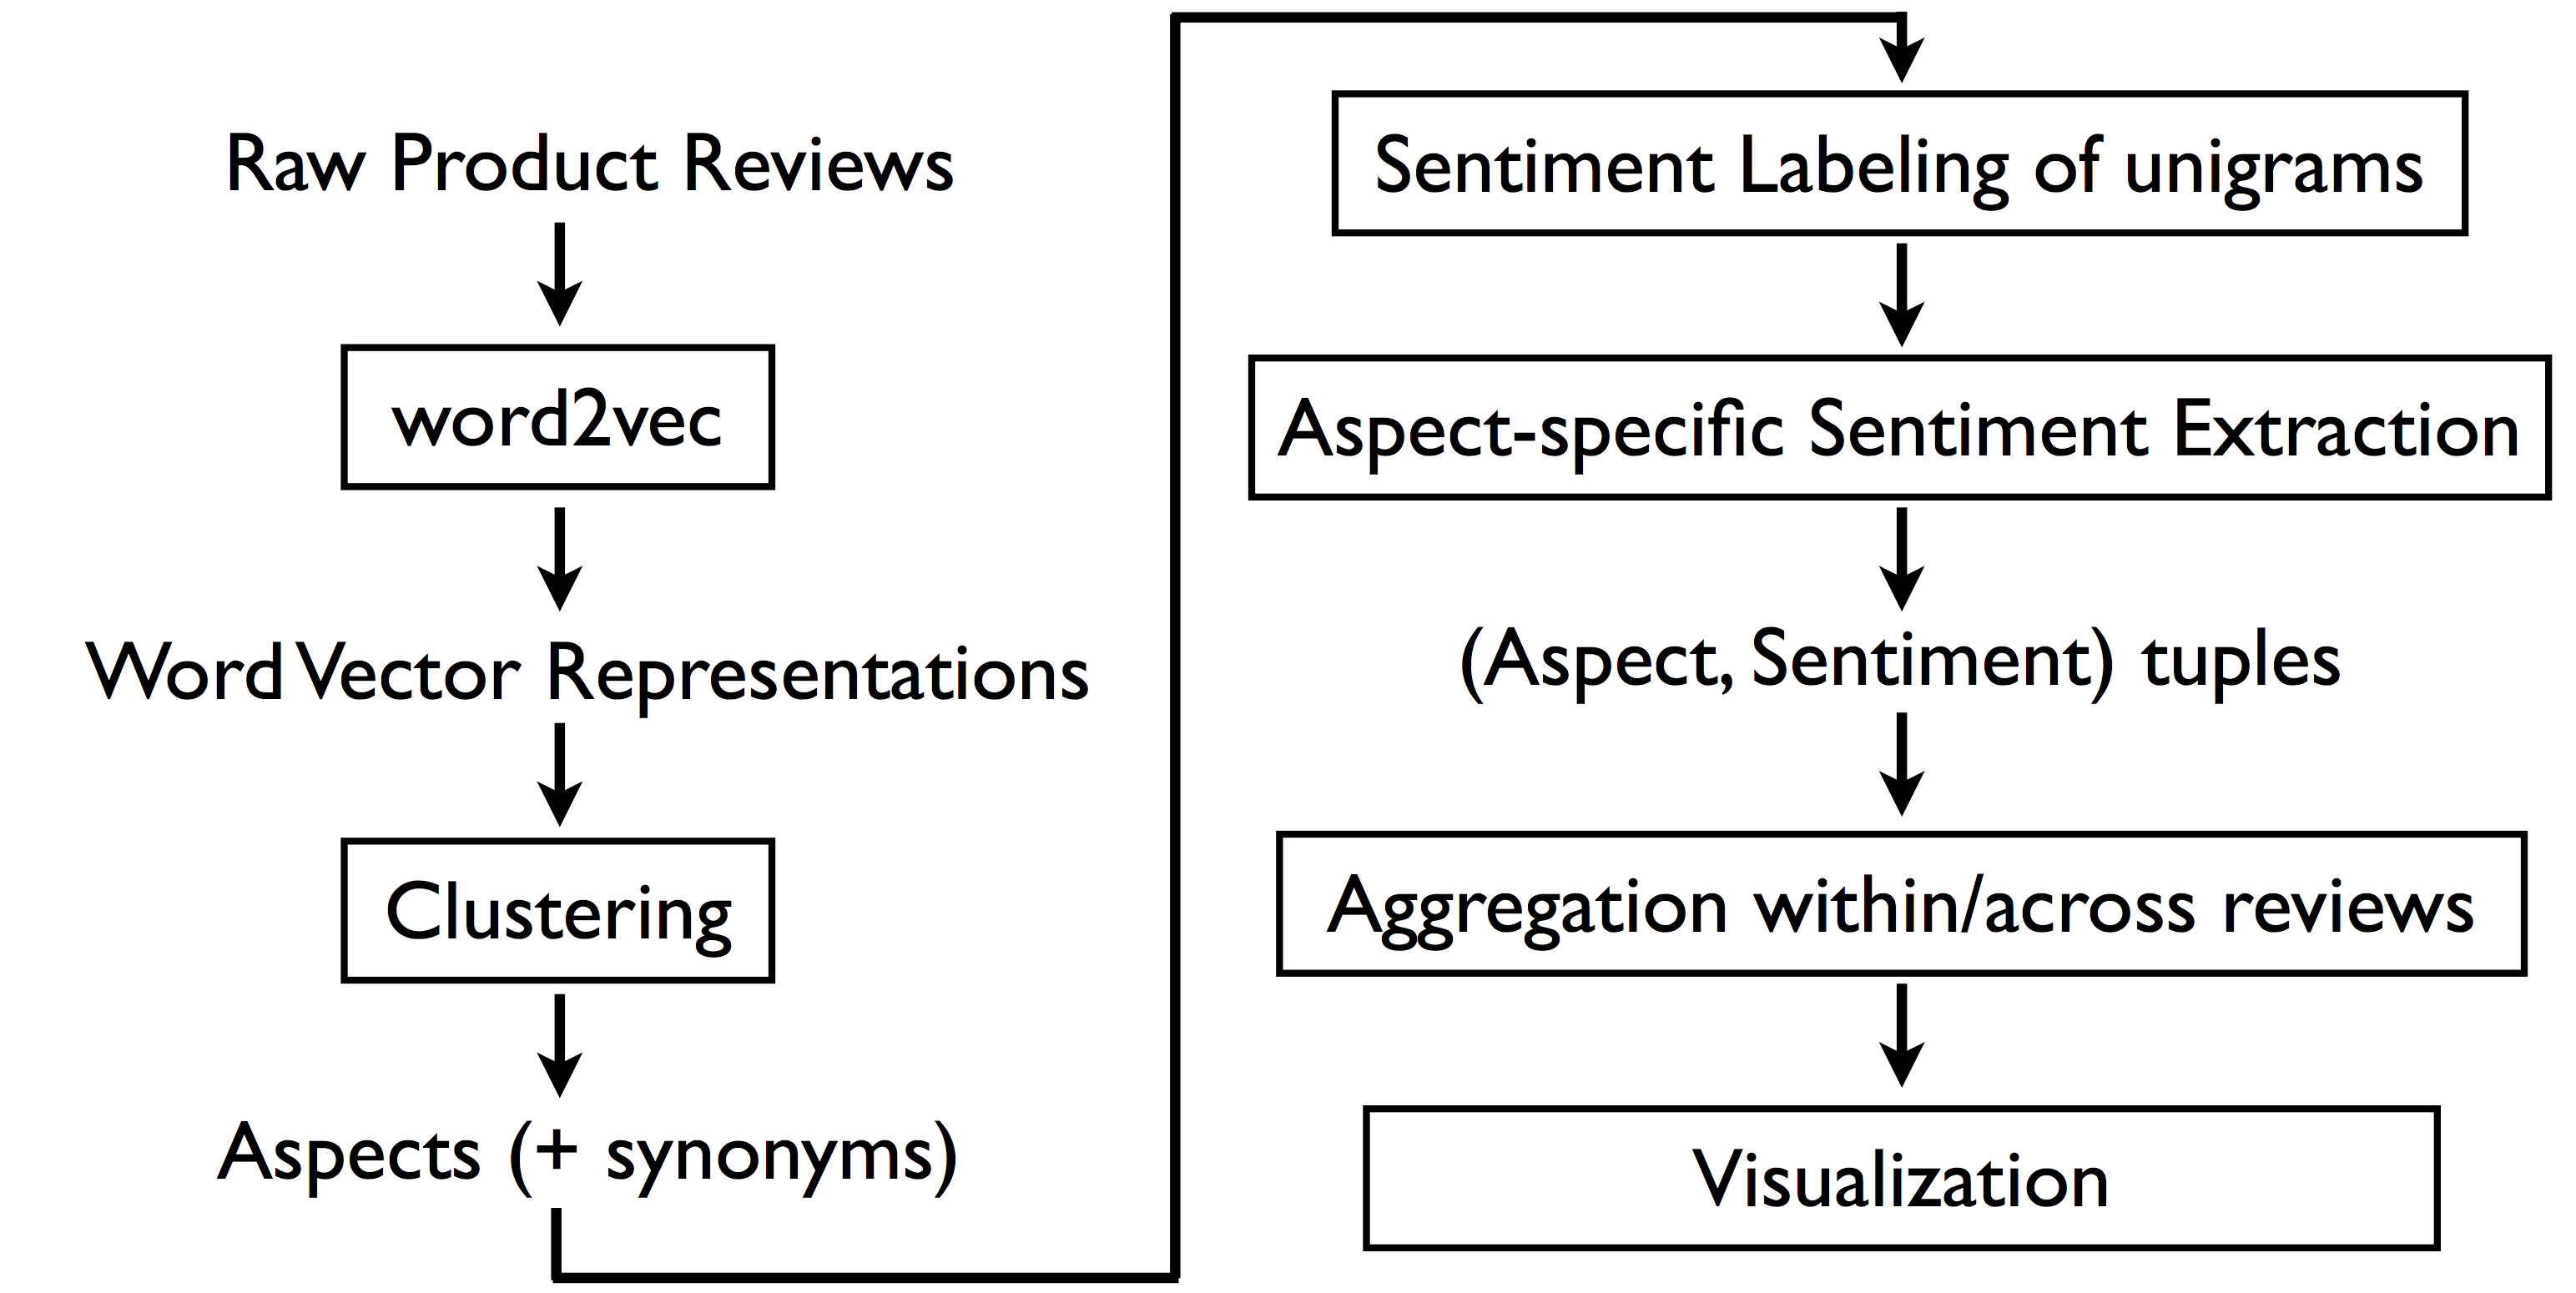
\includegraphics[width=1\columnwidth]{workflow.png}
\end{center}
\caption{Proposed Workflow. Boxed items are processes, while non-boxed items are outputs. The left half of the diagram details unsupervised aspect identification, while the right half of the diagram involves aspect-specific sentiment extraction, summarization and visualization. Except for the Sentiment Labeling and Visualization processes, every other process involves deep learning.}
\label{workflow}
\end{figure}



\subsection{Aspect Identification}

The first part of the project involves an unsupervised approach to generating aspects. First, we run word2vec to obtain a word vector representation of the data. Then, we would perform k-means clustering (or some other clustering algorithm) on the word2vec representations. This would generate clusters of similar words, such as: \{build construction, build quality, durability, etc\}. We can then define the weighted centroid of these clusters as {\bf Aspects}, and the other words in the cluster as relevant synonyms. This allows us to label all the aspect-words in the dataset.


%{\it Desmond and Shane's discussion: it might be counter-intuitive but beneficial to treat Expensive as an attribute (for Price). The NER model will be doing something ``wrong" in labeling an adjective as an entity, but you'll be able to capture the price information when someone says ``expensive".}


\subsection{Aspect-Specific Sentiment Extraction}

An additional pre-processing step would be to label all unigrams with a trained sentiment analysis model. With the aspect-labels from the previous part, we would have a dataset labeled with aspect and (unigram-) sentiment.

Next, we build off and improve on the model in [7] to use a RNTN or improved architecture to extract (aspect, aspect-specific sentiment) tuples from the data.


\subsection{Aspect-Specific Sentiment Aggregation}

The final part of our project involves aspect-specific sentiment aggregation across sentences within a review, and at a further step, aggregating across reviews. We are still currently reading relevant literature (e.g. [8-10]) to come up with ideas on how to optimally construct this. A non-deep learning approach might be to hand-specify features (review length; timing -- more recent reviews might be more important; etc). In contrast, a deep learning proposal would be to have a deep learning network (such as a recursive neural network with individual reviews as tokens) to try to come up with an optimal way of aggregating this information. We plan to scrape professional review websites like Consumer Reports, CNET and/or DPReview, to provide gold standard summary reviews that our model will predict.


An application-related goal would be to have visualization of our output, in terms of a word cloud of important aspects (e.g., sized by word frequency and colored by sentiment), or a bar chart that shows the relevant aspects and their associated sentiment.


%
%\begin{enumerate}
%\item Run word2vec to get an embedded representation
%%\item Start with a small (hand-generated) seed list of attributes (``Entities").
%%	\begin{itemize}
%%	\item Build Construction
%%	\item Price
%%	\item Battery Life
%%	\item ...
%%	\end{itemize}
%\item k means clustering on the word2vec:
%%\item Use the word2vec representation to find similar words/phrases. 
%(This process might also generate adjectives or common phrases used to describe attributes.)
%	\begin{itemize}
%	\item Build Construction, Build Quality
%	\item Price, Cost, (Expensive, Cheap, Affordable)
%	\item Battery Life, (Long-Lasting), Charging
%	\item ...
%	\end{itemize}
%	{\it Desmond and Shane's discussion: it might be counter-intuitive but beneficial to treat Expensive as an attribute (for Price). The NER model will be doing something ``wrong" in labeling an adjective as an entity, but you'll be able to capture the price information when someone says ``expensive".}
%\item Use this list in an NER model to teach it to learn to recognize attributes as a new class of entities.
%\item Next, given that attributes are labelled in the text, we can run sentiment analysis.
%        \begin{itemize}
%	\item Most naively, we can just label all the unigrams. Then, we can just take every sentence, find all the attributes listed in that sentence, and then associate the sentiment of the entire sentence to those attributes.
%	\item More sophisticated models would involve looking at local context and compositionality. Thus, we could run a window (instead of the whole sentence), calculate the sentiment associated with the words in the window (either at the unigram level or at the subtree level, a la Socher et al), and associate that sentiment with the attribute found within the window.
%	\end{itemize}
%\item Then we would have to aggregate sentiment within a review / across reviews.
%\item The output would be a (long and sparse) attribute vector where the $i$-th element is the sentiment associated with the $i$-th attribute:
%        \begin{itemize}
%	\item E.g. attribute$_1$ = build quality, attribute$_2$ = cost
%	\item If product has good build quality but is very expensive, then \\
%	outputAttributeVector = [4, 0, $\ldots$] (scale from 0-4)
%	\end{itemize}
%\item Visualization of output vector.
%\end{enumerate}




%When one is planning a purchase, one usually has to spend time sifting through multiple reviews across many different websites, distilling the information to get (1) ratings for individual attributes (�battery life�), and (2) an overall rating / summary of the information, presented in a �meta-review�. 
%Four separate sub-problems:
%1) Doing POS-tagging and named entity recognition for various product attributes (e.g. battery life, weight, portability, etc) (we�ll probably use off-the-shelf (Stanford NLP) tools for this problem)
%2) Train word2vec representations of said attributes and clustering them (e.g. �build quality� and �construction� can refer to the same attribute)
%3) Extract sentiment based on product attributes
%4) Aggregate this information across multiple reviews (creating a �meta-review�)
%A potential application allows for quick comparisons of various products based on user-generated reviews. Say you are purchasing an Android tablet and are looking at the Samsung Galaxy Tab 4, Nexus 9, Nvidia Shield and other similar products, our system would allow users to identify key attributes of each product (e.g. screen resolution, build quality, battery life, etc) and their associated sentiment, i.e. how positively or negatively do people feel about each product attribute.
%Given the constraints of a class project, we will be limiting our dataset to reviews of electronic consumer products.


%POS and NER: Using off-the-shelf tools
%Clustering entities: cluster learned word2vec representations (e.g. K-NN or distribution-based clustering methods)
%Extract entity-level sentiment: modifying and extending Socher et al (2013)�s model via calculating the sentiment in a window/neighborhood around the named entity, up to the whole sentence.
%Aggregation of sentiment (across multiple sentences, and across multiple reviews): this is perhaps where deep-learning might be extremely useful, but as yet we do not know enough about various deep learning architectures to do this optimally. There are several papers that we identified that might give us some insight (although they don�t use deep learning)




\section{Intermediate/Preliminary Experiments \& Results}
\subsection{Preprocessing} We tokenized our corpus using NLTK's punkt tokenizer [12] for sentence splitting. We then removed all non-alphanumerical characters and replaced all digits with \texttt{DG}. Finally, we performed collocation detection to detect common bigrams.

\subsection{Model Training} We trained three different word2vec models. The most successful model was trained using the CBOW (continuous bag-of-words) model with a window size of 10 and feature dimension size of 300. We also ignored all words with total frequency count below 40 (this helped to remove many typos). We determined the performance of each model by querying the model with various aspects common to electronic products (e.g. "portability", "screen quality", etc).

\subsection{word2vec Results}
We queried our word2vec model and returned the top-10 results based on cosine similarity of the word vectors.

\begin{center}
    \begin{tabular}{ | l | p{9cm} |}
    \hline
    Query & Results \\ \hline
    \texttt{portability} & \texttt{(u'portability,', 0.72859996557235718), (u'compactness', 0.64743077754974365), (u'mobility', 0.60842603445053101), (u'versatility', 0.5763777494430542), (u'simplicity', 0.53962129354476929), (u'lightness', 0.53950369358062744), (u'convenience', 0.53897607326507568), (u'ruggedness', 0.5272858738899231), (u'versatility,', 0.5055851936340332), (u'thinness', 0.49253776669502258)} \\ \hline

	\texttt{contrast} & \texttt{(u'contrast,', 0.65686732530593872), (u'sharpness', 0.62712550163269043), (u'color\_saturation', 0.60933655500411987), (u'saturation', 0.57076853513717651), (u'brightness', 0.5553707480430603), (u'gamma', 0.53090476989746094), (u'shadow\_detail', 0.52805298566818237), (u'color\_accuracy', 0.52408510446548462), (u'dynamic\_range', 0.52167940139770508), (u'black\_levels', 0.51741272211074829)} \\ \hline

	\texttt{tripod} & \texttt{(u'monopod', 0.74430769681930542), (u'tripod,', 0.71975594758987427), (u'ball\_head', 0.70861411094665527), (u'tripods', 0.68399727344512939), (u'ballhead', 0.60356354713439941), (u'manfrotto', 0.59598124027252197), (u'monopod,', 0.58229464292526245), (u'pole', 0.56997144222259521), (u'quick\_release', 0.549965500831604), (u'cold\_shoe', 0.5460544228553772)} \\ \hline
    \end{tabular}
\end{center}

As shown in the table above, words like \texttt{portability} returned many synonyms as well as product aspects that are related to it (e.g. \texttt{ruggedness} and \texttt{simplicity}). We also find that our model is capable of returning aspects that are specific and unique to the product category it is trained on. In this case of electronic products, a query like \texttt{contrast} returned words like \texttt{shadow\_detail}, \texttt{dynamic\_range}, \texttt{black\_levels} and \texttt{gamma}, which are aspects specific to devices like monitor displays and cameras.\\
\\
A query like \texttt{tripod} returned various aspects camera tripods, many of them being features that are non-obvious to the layperson. For instance, \texttt{ball\_head} refers to a ball-type tripod heads and \texttt{quick\_release} refers to quick-release tripod mounts. Many of these queries would otherwise perform poorly if we were to use lexical databases like WordNet.

%We can evaluate the attribute sentiments against the formal ratings provided by CNET or consumer reports. An aggregation of sentiment for individual reviews can also be compared against a user�s overall rating of the product.
%We can evaluate the attribute clustering using standard cluster metrics. A projection to a 2-D space for visualization would also be valuable.


%\begin{figure}[h]
%\begin{center}
%%\framebox[4.0in]{$\;$}
%\fbox{\rule[-.5cm]{0cm}{4cm} \rule[-.5cm]{4cm}{0cm}}
%\end{center}
%\caption{Sample figure caption.}
%\end{figure}

%\begin{table}[t]
%\caption{Sample table title}
%\label{sample-table}
%\begin{center}
%\begin{tabular}{ll}
%\multicolumn{1}{c}{\bf PART}  &\multicolumn{1}{c}{\bf DESCRIPTION}
%\\ \hline \\
%Dendrite         &Input terminal \\
%Axon             &Output terminal \\
%Soma             &Cell body (contains cell nucleus) \\
%\end{tabular}
%\end{center}
%\end{table}


\subsubsection*{Acknowledgments}

We would like to acknowledge funding for computing resources provided by the Deep Social Learning Lab at Stanford.

\subsubsection*{References} % chronological. any citation style is acceptable, as long as it's consistent. Use APA

\small{

[1] Titov, I., \& McDonald, R. T. (2008). A Joint Model of Text and Aspect Ratings for Sentiment Summarization. In {\it ACL} (Vol. 8, pp. 308-316).

[2] Jo, Y., \& Oh, A. H. (2011). Aspect and sentiment unification model for online review analysis. In Proceedings of the fourth ACM international conference on Web search and data mining (pp. 815-824). ACM.

[3] Brody, S., \& Elhadad, N. (2010). An unsupervised aspect-sentiment model for online reviews. In {\it Human Language Technologies: The 2010 Annual Conference of the North American Chapter of the Association for Computational Linguistics} (pp. 804-812). Association for Computational Linguistics.

[4] Engonopoulos, N., Lazaridou, A., Paliouras, G., \& Chandrinos, K. (2011). ELS: a word-level method for entity-level sentiment analysis. In {\it Proceedings of the International Conference on Web Intelligence, Mining and Semantics}


[5] Moilanen, K., \& Pulman, S. (2009). Multi-entity Sentiment Scoring. In {\it Recent Advances in NLP} (pp. 258-263).

[6] Socher, R., Perelygin, A., Wu, J. Y., Chuang, J., Manning, C. D., Ng, A. Y., \& Potts, C. (2013). Recursive deep models for semantic compositionality over a sentiment treebank. In {\it Proceedings of the conference on Empirical Methods in Natural Language Processing (EMNLP)} (Vol. 1631, p. 1642).

[7] Lakkaraju, H., Socher, R, \& Manning, C. (2014). Aspect Specific Sentiment Analysis using Hierarchical Deep Learning. {\it NIPS Workshop on Deep Learning and Representation Learning}



[8] Ghose, A., \& Ipeirotis, P. G. (2007). Designing novel review ranking systems: predicting the usefulness and impact of reviews. In {\it Proceedings of the Ninth international conference on Electronic commerce} (pp. 303-310). ACM.

[9] Chen, P. Y., Dhanasobhon, S., \& Smith, M. D. (2008). All reviews are not created equal: The disaggregate impact of reviews and reviewers at Amazon.com. Available at SSRN: http://ssrn.com/abstract=918083 

[10] Dai, W., Jin, G. Z., Lee, J., \& Luca, M. (2012). Optimal aggregation of consumer ratings: an application to Yelp.com (No. w18567). National Bureau of Economic Research. 


[11] McAuley, J., Targett, C., Shi, J., \& van den Hengel, A. (2015). Image-based recommendations on styles and substitutes. {\it ACM Special Interest Group on Information Retrieval (SIGIR)}

[12] Bird, Steven, Loper, E. and Klein, E. (2009). Natural Language Processing with Python. O’Reilly Media Inc.



%% this paper isn't that relevant. it's an evaluation system.
%[2] Ward, C. B., Choi, Y., Skiena, S., \& Xavier, E. C. (2011). Empath: A framework for evaluating entity-level sentiment analysis. In {\it Emerging Technologies for a Smarter World (CEWIT), 2011 8th International Conference \& Expo}. (pp. 1-6). IEEE.


%
%Wang, H., Lu, Y., & Zhai, C. (2010, July). Latent aspect rating analysis on review text data: a rating regression approach. In Proceedings of the 16th ACM SIGKDD international conference on Knowledge discovery and data mining (pp. 783-792). ACM.
%
%Yatani, K., Novati, M., Trusty, A., & Truong, K. N. (2011, May). Review spotlight: a user interface for summarizing user-generated reviews using adjective-noun word pairs. In Proceedings of the SIGCHI Conference on Human Factors in Computing Systems (pp. 1541-1550). ACM.



}

\end{document}
